\documentclass{article}
\usepackage[utf8]{inputenc}

\title{Assignment-4\\Fork assignment-3}
\author{Subash Mylraj \\(CED18I051) }
\date{16 September 2020}

\usepackage{geometry}
 \geometry{
 a4paper,
 total={170mm,257mm},
 left=20mm,
 top=10mm,
 }

\usepackage{longtable}
\usepackage{graphicx}
\usepackage{listings}
\usepackage{xcolor}

\begin{document}

\maketitle

\lstset{
  language=c,
  aboveskip=3mm,
  belowskip=3mm,
  showstringspaces=false,
  columns=flexible,
  basicstyle={\small\ttfamily},
  numbers=none,
  numberstyle=\tiny\color{gray},
  keywordstyle=\color{blue},
  commentstyle=\color{dkgreen},
  stringstyle=\color{mauve},
  breaklines=true,
  breakatwhitespace=true,
  tabsize=3
}

\definecolor{dkgreen}{rgb}{0,0.6,0}
\definecolor{gray}{rgb}{0.5,0.5,0.5}
\definecolor{mauve}{rgb}{0.58,0,0.82}

\section*{Question 3: Develop a C program to count the maximum number of processes that can be created using fork call.}
\bigskip

\textbf{\Large Code:}
\smallskip
\par\noindent\rule{\textwidth}{0.4pt}
\lstinputlisting[language=c]{src/3.c}
\par\noindent\rule{\textwidth}{0.4pt}

\bigskip
\noindent
\textbf{\Large Explanation: } \\

	This code creates child processes in an infinite loop till 
	it reaches a point when it cannot create anymore processes.
	This limit can be assumed as the cap on the number of processes
	that can be created. \\

	To avoid the issue of child processes calling fork repeatedly,
	the child processes are made to sleep for a time of 10 seconds.
	So essentially, this program finds the total number of processes
	that can be created in about 10 seconds (its a bit more than 10
	seconds as there is time taken for context switching and other 
	statements). Increasing the sleep time for each process, produced
	similar results.


\pagebreak
\bigskip
\noindent
\textbf{\Large Output:}

\begin{figure}[h]
	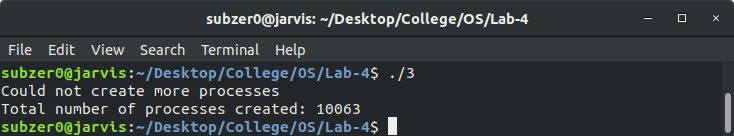
\includegraphics[width=\textwidth]{output/3.png}
\end{figure}
\bigskip
\bigskip
\bigskip

\bigskip


\section*{Question 4: Develop your own command shell [say mark it with @] that accepts user commands (System or User Binaries), executes the commands and returns the prompt for further user interaction. Also extend this to support a history feature (if the user types !6 at the command prompt; it shud display the most recent execute 6 commands). You may provide validation features such as !10 when there are only 9 files to display the entire history contents and other validations required for the history feature;}
\bigskip

\textbf{\Large Code:}
\smallskip
\par\noindent\rule{\textwidth}{0.4pt}
\lstinputlisting[language=c]{src/4.c}
\par\noindent\rule{\textwidth}{0.4pt}

\bigskip
\noindent
\textbf{\Large Explanation: } \\
% \bigskip
  \\This code creates a new terminal interface. Any command that is located in the
  $/bin/$ directory will work. Sadly piping logics do not work on this terminal. The 
  command $exit$ can be used to exit the terminal. Though it is to be noted that, 
  this command is not called through exec statements. \newline \\
  History of the last 10 commands can be displayed by typing $!$. Further, typing $! 5$
  shows the last 5 commands used. Typing a value more than 10 will only print the 
  last 10 commands used. \newline \\
  Colours were added using $\setminus 033$ in printf statements. \newline \\
  Directories can be changed by using the cd command. This command is not called
  through exec calls rather by calling the chdir functions. The prompt displays the
  current username and hostname using $gethostname()$ and $getlogin\_r()$ functions. The
  current working directory information is obtained by using the $getcwd()$ functinon.

\bigskip
\noindent
\textbf{\Large Output:}

\begin{figure}[t]
	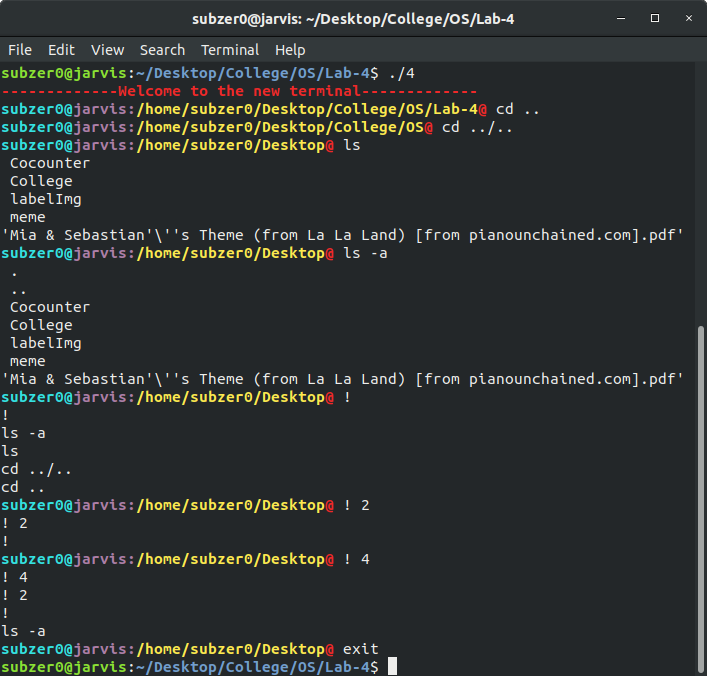
\includegraphics[width=\textwidth]{output/4.png}
\end{figure}
\bigskip
\bigskip
\bigskip

\bigskip

\end{document}